%%% gssa.tex --- 


\section{Background}

In past years, with the development of genomic data in close related species, an effort was made in order to detect signals of selective pressure by applying methods that have been developed since \cite{Kimura1985} based on observations of significant deviation from neutrality for a given gene. These methodologies conceived for the study of a single gene were successfully able to detect genes escaping neutrality ($\omega \ne 1$ see Equation \ref{eq:omega} page \pageref{eq:omega}), and in particular positively selected genes (with $\omega > 1$)  \cite{Arbiza2006,Bakewell2007,Bustamante2005,Clark2003,Nielsen2005}. However none of those works were able to find, within the groups of genes detected to be under positive selection, a significant enrichment of a given functional trait. It is true that taking all those results together, assiduous readers could perceive functional patterns raising from all those studies. Functional terms related to \textit{Sensory perception}, \textit{Immune response} or \textit{Regulation of transcription} were present in almost all genomic studies of positive selection conducted in primates or rodents.


measured in coding regions using the  Statistical methods to test for neutrality \cite{Nielsen2001}, are currently used without considering if genes works independently or associated to others to produce a single phenotypic response. In this sense we are applying pre-genomics concepts and methods to genomics data. The current paradigm for large scale analysis of adaptation consists in a two steps framework: first, the search for a list of genes (in a gene-by-gene framework analysis) with a statistical significant signal of positive selection ($\omega > 1$), and second, the search for over-represented functional classes of genes in this list. Although it is logically consistent, it has been noted that this kind of strategy causes an enormous loss of information due to the large number of false negatives that are accepted in order to preserve a low ratio of false positives necessary when genomics data is considered~\cite{Al-Shahrour2007,Al-Shahrour2005a,Al-Shahrour2006,Subramanian2005}.

Genes do not operate alone within the cell, but in a intricate network of interactions that we have only recently started to envisage~\cite{Stelzl2005}. It is a widely accepted fact that coexpressing genes tend to be fulfilling common roles in the cell~\cite{Lee2003}. Moreover, coexpression seems to occur, in many cases, in contiguous chromosomal regions~\cite{Caron2001} and furthermore, recent evidences suggest that functionally related genes map close in the genome, even in higher eukaryotes~\cite{Hurst2004}. Many higher-order levels of interaction are continuously being discovered and even complex traits, including diseases, have started to be considered from a systems biology perspective~\cite{Ideker2008,Vamathevan2008}.

Recent methodology was proposed to circumvent the classical two-step analysis as a new attempt to test for selective signatures across species at genome-scale level~\cite{Shapiro2008} Using the deviations of the expected rates of evolution for a large group of genes in a group of gamma proteobacteria, the authors conclude that the coherence of selective patterns suggests that the genomic landscape is organized into functional modules even at the level of natural selection.

The hypothesis we aim to test in this study is not about individual genes, but about functional classes. Mutations occur on single genes but natural selection acts on phenotypes by operating on whole sub-cellular systems. Mutations in genes either remain finally fixed or disappear because of their beneficial or disadvantageous effect on individual fitness, respectively. This effect on the function of individual proteins can only be understood in the context of the system (e.g. a pathway, GO functional roles, etc.) in which the proteins are involved. If a list of genes arranged by some parameter that accounts for their evolutionary rates is examined, it is expected that genes belonging to pathways or functional classes favored or disfavored by selection will tend to appear towards the extremes.

This approach circumvents the implicit assumption posed by the two-step analysis described above assuming by that the gene is the only target of selection. If natural selection works by means of minor quantitative effects of many different changes distributed along different gene products most of them working together in a few number of systems (GO functional terms, biochemical pathways and/or interactome modules) we expect to find: \begin{inparaenum}[ 1-] \item correlated nonsynonymous rate changes associated to these functions , \item synonymous rate changes not necessarily associated to the same functions, \item a higher number of significant functions than those discovered in the classical two-step approach.\end{inparaenum}

In the first part of this paper we extend the classical two-step approach previously reported by us for human and chimp \cite{Arbiza2006}, to rat and mouse now considering a set of XXXX orthologous genes of human, chimpanzee, mouse, rat and dog. The objective is to compare the classical two-step approach with the new system approach developed in the second part of the paper. In both cases we search for differences in evolutionary rates differentiating positive selection from relaxation along the branches of the phylogeny of the species.

\section{Results}

\subsection{Gene-set selection analysis on functional modules}

Mammals, represented by human, chimpanzee, rat and mouse, and five Drosophila genomes were studied. For each species, genes were ranked into four lists according to the estimation of \begin{inparaenum}[i\upshape-] \item synonymous (dS), \item nonsynonymous (dN) rates of substitution, \item selective pressures ($\omega$ = dN/dS), and \item the change of selective pressures between (A) ancestor and (D) descendant species ($\Delta\omega$D = $\omega$D-$\omega$A) along the phylogeny \fref{fig:phylogeny}{}\end{inparaenum}. Maximum likelihood (ML) estimates of evolutionary variables were performed using a free-ratio branch model \cite{Yang2007}. As such, four lists containing 12,543 and 9,240 orthologous genes in mammals in Drosophila species were obtained for the analyzes, respectively. GSSA was conducted using a total of 1,394/199 and 1,331/116 GO/KEGG terms in mammals and Drosophila species respectively. GSSA is performed in five different steps (S1 to S5 in \fref{fig:gssa_met}{} on page \pageref{fig:gssa_met} in Section \ref{sec:gssa_mat-met}). First, the method ranks all genes within a genome (G) according to one of the alternative evolutionary variables (dS, dN, $\omega$ and $\Delta\omega$). Second, genes are associated (dark dots) to different functional categories (GO or any other functional term). Note that a single gene can be associated with multiple functions (yellow bar in Figure 2). Third, for each functional category a total of 30 partitions are established along the list of ranked values \cite{Al-Shahrour2007}, \cite{Al-Shahrour2005a}. Fourth, for each partition GSSA computes a two-tailed Fisher's exact test and reports significant over or under represented functional classes comparing the upper side (A) and the lower side (B) of the list. Finally, p-values are corrected for multiple testing (FDR). Throughout the manuscript only p-values for partitions with the highest confidence were reported after FDR.

The application of GSSA to lists of genes ranked by dS, dN, $\omega$ and the $\Delta\omega$ values yielded a large number of functional modules (defined by GO and KEGG annotations) with rates that were significantly skewed toward the extremes of the lists (\tref{tab:gssanum_perc}) in mammal and \textit{Drosophila} species. For instance, 11\% of GO terms, and 15\% of KEGG pathways contain genes with biased distribution of rates towards the top of the ranked list, and found statistically significant at high $\omega$ ratio (SH$\omega$, 5\% false-discovery rate, FDR) in mammals. Alternatively, 4.1\% and 2.6\% of GO terms and KEGG pathways were found with significantly high values of $\omega$ (SH$\omega$) in \textit{Drosophila}, respectively.

\begin{table}[htbp]
\begin{center}
\begin{tabular}{ l l l l l l }
\hline
 &  & \multicolumn{ 2}{c}{\textbf{SH*}} & \multicolumn{ 2}{c}{\textbf{SL*}} \\  \cline{ 3- 4} \cline{4-6}
 &  & \multicolumn{1}{c}{\textbf{KEGG }} & \multicolumn{1}{c}{\textbf{GO }} & \multicolumn{1}{c}{\textbf{KEGG }} & \multicolumn{1}{c}{\textbf{GO}} \\ \hline
\multicolumn{ 1}{l}{Mammals} &  dS  &  15 (1.9)    &  187 (3.3)   &  12 (2.1)    &  364 (6.5) \\
\multicolumn{ 1}{l}{} &  dN  &  145 (18.2)  &  708 (12.6)  &  230 (28.9)  &  1,839 (32.9) \\
\multicolumn{ 1}{l}{} & $\omega$ &  123 (15.5)  &  649 (11.6)  &  206 (25.9)  &  1,675 (30.0) \\
\multicolumn{ 1}{l}{} & $\Delta\omega$ &  64 (8.0)    &  421 (7.5)   &  107 (13.4)  &  818 (14.7) \\ \hline
\multicolumn{ 1}{l}{Drosophilas} &  dS  &  18 (3.1)    &  104 (1.5)   &  26 (4.5)    &  1,263 (18.9) \\
\multicolumn{ 1}{l}{} &  dN  &  31 (5.3)    &  276 (4.1)   &  26 (4.5)    &  2,097 (31.5) \\
\multicolumn{ 1}{l}{} & $\omega$ &  15 (2.6)    &  213 (4.1)   &  24 (4.1)    &  1,321 (19.8) \\
\multicolumn{ 1}{l}{} & $\Delta\omega$ &  2 (0.3)     &  143 (2.1)   &  7 (1.2)     &  184 (2.8) \\ \hline
\end{tabular}
\end{center}
\caption[Numbers and percentages of functional modules with significant results after GSSA.]{Numbers and percentages of functional modules with significant results after GSSA. For Significantly High (SH) and Significantly Low (SL) results.}
\label{tab:gssanum_perc}
\end{table}

\tref{tab:gssanum_perc} also reveals that functional modules with genes changing at significantly low $\omega$ ratios (SL$\omega$), and therefore showing a distribution shifted towards the bottom of the ranked list (see Figure 2), were more frequent than modules under the significantly high $\omega$ (SH$\omega$). This observation is in agreement with the fact that purifying selection is the predominant form of selection in biological systems. Moreover, in support of the slightly neutral character of synonymous mutations, and the effects of population size in the final outcome of selection \cite{Lynch2007} GSSA results show a higher number of significant deviations of dS in \textit{Drosophila} rather than in mammals.

Only a minor proportion of functional terms changed significantly at higher or lower rates relative to estimates of the corresponding ancestral lineages. Specifically, increased or decreased $\omega$ values on the external branches (recorded by positive and negative values of $\Delta\omega$) were observed for only half of the cases where a significant increase or decrease of $\omega$ was identified in mammals and Drosophilas. This observation points out the conservative character of the selective constraints in functional related groups of genes during evolution.

A summary of the results of the GSSA for mammals and \textit{Drosophilas} is shown in \fref{fig:tab_gssa}{} (see Figures S1 to S4 for a complete description of results after GSSA in mammals and \textit{Drosophila} species). The figure shows that GSSA has the power to detect many functional changes in evolutionary rates within a substantial number of functional categories. Although the rough pattern shows similar evolutionary constraints in groups of genes between the two main clusters of species, important differences were also detected within them. For instance, functional terms associated to neurological process and sensory perception clearly contrasted between primates and rodents (\fref{fig:tab_gssa}{-A}). While most of these terms are associated to a significant relative increase in rates from the common ancestor of primates (+$\Delta\omega$), all the changes observed in rodents were due to the relative increase of the selective constraints (-$\Delta\omega$) probably due to the effects of purifying selection from the common ancestor. Alternatively, functional modules associated to Immunity and Defense response evolved at significantly higher rates than expected in rodents, but decreased significantly in relation to the ancestral rates in primates. Such functional differences between primates and rodents were previously observed when pooling groups of species \cite{Kosiol2008a}. Other functional modules such as \textit{Development}, and \textit{Transcription/Transduction} comparatively evolved at very low dN and $\omega$ ratio but experienced a higher relaxation of the ancestral constraints (+$\Delta\omega$) in primates than in rodents. Moreover, significant differences in rates can be detected between human and chimpanzee (Ha04360: \textit{Axon guidance}, Ha04610: \textit{Antigen processes and presentation}, GO0007268: \textit{synaptic transmission}, among others), and between mouse and rat (GO0007186: \textit{G-protein coupled receptor protein signaling pathway}, and Ha04310: \textit{Wnt signaling pathway}, among others).


\begin{FPfigure}
\centering 
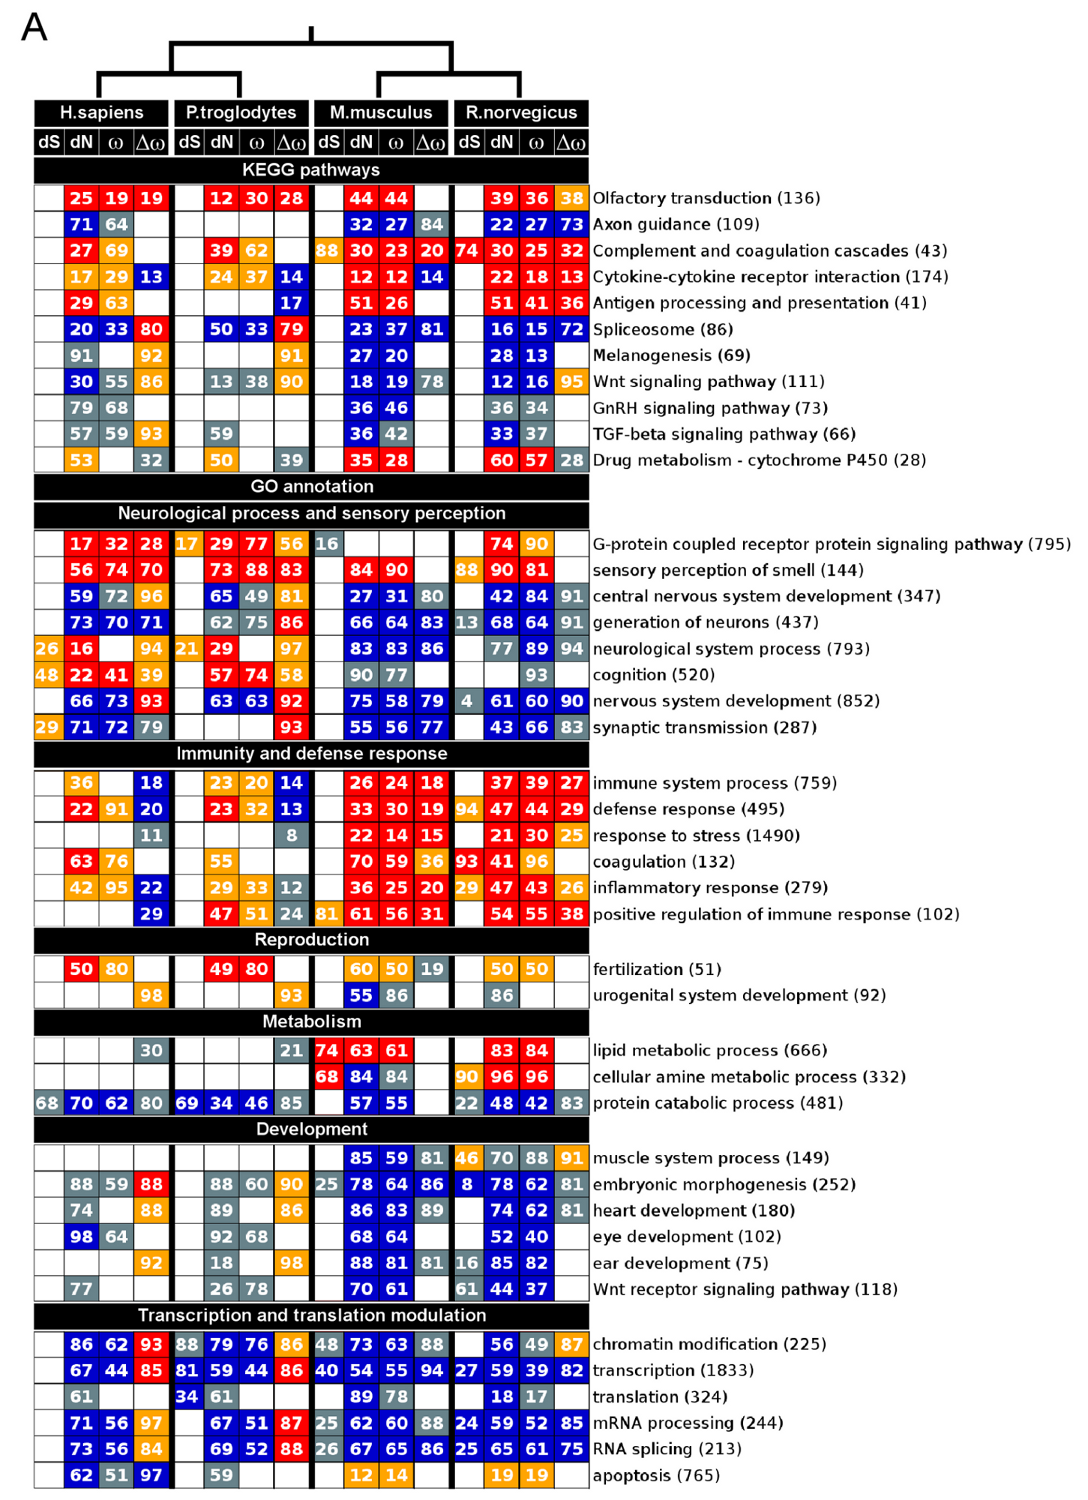
\includegraphics[width=\textwidth]{tex_source/figures/gssa/table_mammals_2.png}
\caption[GSSA of evolutionary variables.]{{\bf GSSA of evolutionary variables.} \\The figure shows a selection of GO terms and KEGG pathways with significant and not significant deviations after GSSA of evolutionary rates in mammals (A) and Drosophila (B) species. Colored boxes represent functional modules with genes significantly accumulated at the corresponding extremes of the ranked list as explained in Figure 2. The number inside each box represents the percentage of the total number of genes of the functional module (in parenthesis) that contribute to its significance. Here we reported the numbers of the first significant partition after FET and FDR. Topologies represent the phylogenetic relationships of species.} 
\label{fig:tab_gssa}
\end{FPfigure}
\begin{figure}
\centering 
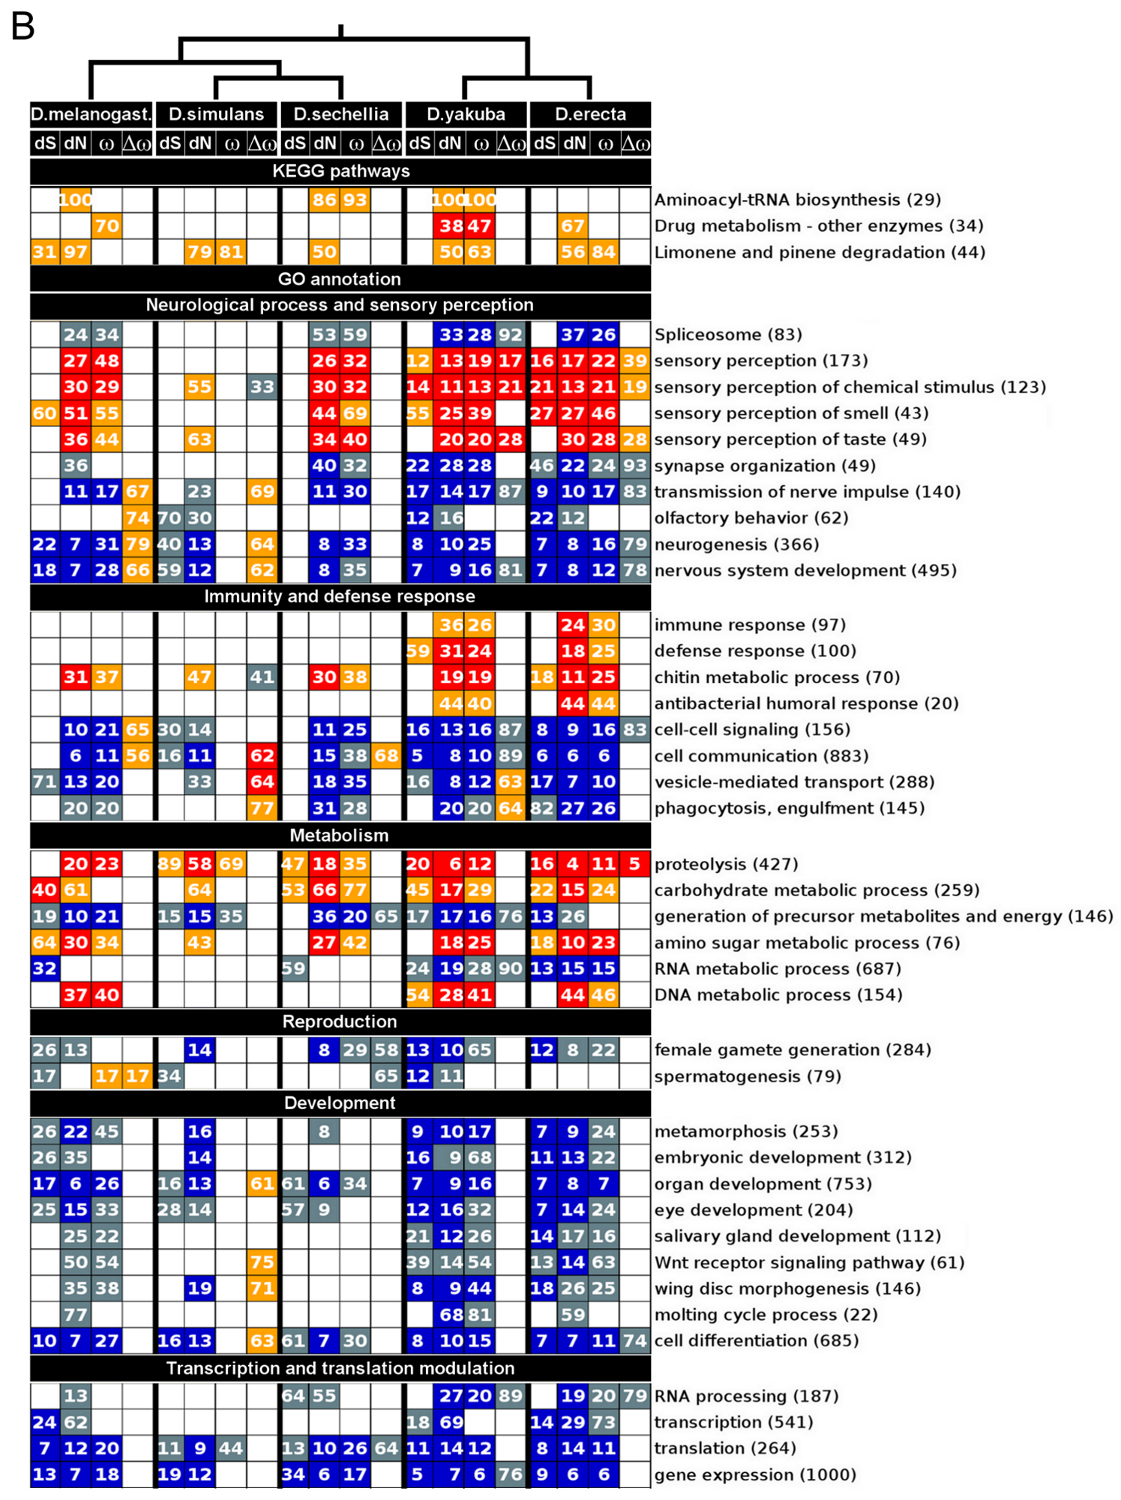
\includegraphics[width=\textwidth]{tex_source/figures/gssa/table_flies_2.png}
\end{figure}

In addition, most of the GO terms significantly associated to high dN and $\omega$ in Drosophilas were unevenly distributed within the two clusters of the phylogeny (\fref{fig:tab_gssa}{-B}). GO terms such as sensory perception, defense response, immune response and metabolic process, among others, presented a remarkable divergence in the monophyletic groups of \textit{D. erecta} and \textit{D. yakuba} but they were not observed in \textit{D. sechellia}, \textit{D. melanogaster} and \textit{D. simulans}. Most of GO terms from \textit{Development}, \textit{Transcription} and \textit{Translation} (\fref{fig:tab_gssa}{-A and -B}) were significantly accumulated towards the extremes of the lists corresponding to the lowest rates of substitutions, suggesting they are significantly constrained by strong purifying selection (5\% FDR) in both taxa.

The fact that most of the functional modules under selection (SH$\omega$ and SL$\omega$) correlate with changes in dN, suggests that selective pressures are mainly driven by nonsynonymous rather than by synonymous substitutions during evolution. Moreover, according to the expectation of the nearly neutral theory, a low but still considerable number of significant associations of functional modules to dS were found in \textit{Drosophila} (19.5\%) and rodents (11.3\%), while in primates (6.4\%), where population sizes are known to be smaller, the number of significant modules was smaller \cite{Petit2009}.

The strategy presented here lead to detect significant patterns of increments and decrements modeled by natural selection in evolutionary rates of functional groups of genes. This pattern is consistent with the hypothesis that natural selection acts on phenotypes by the combined action of many functional related genes. Moreover, this functionally based approach identified with statistical significance, and on individual species, all the functional modules previously found significantly enriched by positively selected genes and therefore the main targets of adaptive biological functions in species \tref{tab:gssa_compare}. Although GSSA is not a test for positive selection, it is evident that functional modules containing PSGs can be significantly detected by this method on individual species. In the next section we will analyze the relative contribution of PSGs to the statistical differentiation of functional modules in genomes.


\rowcolors{2}{white}{gray}
\begin{FPtable}
\caption[Functional enrichment results using gene-by-gene and gene-set approaches.]{\textbf{Functional enrichment results using gene-by-gene and gene-set approaches.}\\The table depicts some selected biological functions enriched by PSGs as cited in references 1 to 7, and the corresponding significant result observed after GSSA of $\omega$ values. References 1 to 7 correspond to cites 6, 7, CSAC, 4, 5, 9 and 8 in the manuscript, respectively. Abbreviations: SHv: statistically significant high v values; SLv: statistically significant low v values; H: \textit{H. sapiens}; C: \textit{P. troglodytes}; Pr: primates; M: \textit{M. musculus}; R: \textit{R. norvegicus}; Ro: rodents; mel: \textit{D. melanogaster}; sim: \textit{D. simulans}; sec: \textit{D sechelia}; yak: \textit{D. yakuba}; ere: \textit{D. erecta}; Ds: \textit{Drosophila} species.\\
*: p=0.05;\\
** p=0.001. CSAC: Chimpanzee Sequencing and Analysis Consortium, Nature. 2005 vol. \textbf{437} (7055) pp. 69-87.}
\resizebox{410pt}{!}{%
  \begin{tabular}{ p{8.5cm} p{0.8cm} p{0.8cm} p{0.5cm} p{0.8cm} p{0.5cm} p{0.85cm} p{0.5cm} p{8cm}}
  \hline
  \textbf{Biological process} & \multicolumn{ 7}{c}{\textbf{Enrichment in PSGs}} & \textbf{GSSA: Functional category with significantly} \\ \hline
   & \textbf{1} & \textbf{2} &  \textbf{3} & \textbf{4} & \textbf{5} & \textbf{6} & \textbf{7} & \multicolumn{1}{r}{\textbf{HIGH rates of omega}} \\ \hline
  Olfaction/Sensory perception of smell & H & Pr** &  &  &  & Pr** &  & H**, C**, M**, R**, mel*, sec*, ere**, yak** \\
  Chemosensory perception & H & Pr** &  &  &  &  &  & H**, C**, M**, R**,  mel**, sec**, ere**, yak** \\
  G-protein-mediated signaling & H &  &  &  & H & Pr** &  & H**, C**, R* \\
  DNA/nucleic acid metabolism &  &  &  & C &  &  & Dr & C*, M**, R**, mel**, yak**, ere* \\
  Amino acid metabolism & H, C &  &  &  &  &  & Dr & M**, R** \\
  Proteolysis &  &  &  &  &  &  & Dr & M**, R**, mel**, sim*, sec*, yak**, ere** \\
  Fatty acid/Lipid metabolism &  &  &  &  & H &  & Dr & M**, R** \\
  Carbohydrate metabolism &  &  &  &  &  &  & Dr & sec*, yak*, ere* \\
  Adult reproduction and gametogenesis &  &  &  &  &  &  & Dr & sec* \\
  Spermatogenesis and motility &  & Pr* & Pr &  &  &  &  & H*, M*, mel* \\
  Immune response &  & Pr** &  & H, C &  & Ro** &  & C*, M**, R**, yak*, ere* \\
  Inflammatory response &  &  &  &  &  & Ro** &  & H*, C*, M**, R** \\
  Defense response &  &  &  &  &  & Ro** &  & H*, C*, M**, R**, yak**, ere* \\
  Response to wounding &  &  &  &  &  & Ro** &  & H*, M**, R** \\
  Hummoral imm. resp. mediated by circulating Ig &  &  &  &  &  & Ro** &  & M**, R** \\
  T-cell-mediated immunity &  & Pr** &  &  &  &  &  & M* \\
  Natural killer-cell-mediated immunity &  & Pr* &  &  &  &  &  & R* \\
  B-cell- and antibody-mediated immunity &  & Pr* &  &  &  &  &  & M**, R** \\
  Response to pest, pathogen, or parasite &  &  &  & H &  &  &  & C*, M**, R**, yak*, ere* \\
  Stress response &  &  &  &  & C & Ro** &  & M**, R** \\
  Response to external stimulus &  &  &  &  &  & Ro** &  & M**, R* \\
  Sensory Perception & H & Pr** &  & H &  & Pr** &  & H**, C**, M*, mel**, sec**, yak**. ere** \\
  Cell surface receptor-mediated signal trasnduction & H &  &  &  &  & Pr** &  & C* \\
  Cell adhesion & H &  &  &  &  &  &  & R* \\
  Amino acid transport &  &  & Pr &  &  &  &  & M* \\
  Protein amino acid glycosylation &  &  & Pr &  &  &  &  & M* \\
  Amino acid transport & C &  &  &  &  &  &  & M* \\ \hline
  \multicolumn{9}{r}{\textbf{LOW rates of omega}} \\ \hline
  Sensory Perception & H & Pr** &  & H &  & Pr** &  & R* \\
  Cell surface receptor-mediated signal trasnduction & H &  &  &  &  & Pr** &  & mel*, yak*, ere* \\
  Cell adhesion & H &  &  &  &  &  &  & H**, C**, mel**, ere* \\
  Amino acid transport &  &  & Pr &  &  &  &  & R* \\
  Protein amino acid glycosylation &  &  & Pr &  &  &  &  & H* \\
  Amino acid transport & C &  &  &  &  &  &  & C* \\
  Hearing / Perception of sound & H &  & Pr &  &  &  &  & M*, R* \\
  Neurological process &  &  &  &  &  & Pr** &  & M**, R**, yak*, ere* \\
  Synaptic transmission &  &  & Pr &  &  &  &  & H**, M**, R**, mel**, sec**, ere**, yak** \\
  Signal transduction/intracellular signaling cascade & H, C &  & Pr &  &  &  & Dr & H**, C**, M**, R**, dmel**, dsec*, dyak**, dere** \\
  Ion transport & H &  &  &  & H &  & Dr & H*, M**, R**, mel*, sec*, ere* \\
  Potassium ion transport &  &  & Pr &  &  &  &  & H*, C*, M**, R** \\
  Inorganic anion transport &  &  & Pr &  &  &  &  & M*, R* \\
  Intracellular protein traffic & H &  &  &  &  &  &  & H**, C**, M**, R**, mel*, sec**, yak**, ere* \\
  Transport &  &  &  &  &  &  & Dr & mel**, sec**, ere**, yak** \\
  Protein transport &  &  &  & H &  &  & Dr & H*, C**, M**, R**, mel**, sim*, sec**, ere**, yak** \\
  Metabolism of cyclic nucleotides & H &  &  &  &  &  &  & M*, R* \\
  Protein metabolism \& modification &  &  &  & H, C & C &  & Dr & H**, C**, M**, R**, ere*, yak* \\
  Phosphate metabolism/phosphorylation &  &  &  & H, C &  &  & Dr & H*, C*, M**, R**, mel*, sec**, yak**, ere* \\
  Purine metabolism & C &  &  &  &  &  &  & M*, R*, sec** \\
  Carbohydrate biosynthesis &  &  & Pr &  &  &  &  & M**, R* \\
  Cation transport & H &  &  &  &  &  &  & H*, M**, R** \\
  Nervous system development &  &  &  &  &  &  & Dr & H*, M**, R**, mel**, sec*, yak**, ere** \\
  Skeletal development & C &  &  &  &  &  &  & M**, R** \\
  Organ development &  &  &  &  &  &  & Dr & H*, M**, R**, mel**, sec*, yak**, ere** \\
  Post-embryonic development &  &  &  &  &  &  & Dr & M*, mel*, yak**, ere* \\
  Embryonic development &  &  &  &  &  &  & Dr & H**, C*, M**, R**, yak*, ere* \\
  Ectoderm development &  &  &  &  & H &  &  & C*, M*, R*, mel*, yak*, ere* \\
  Cell proliferation and differentiation & C &  &  &  &  &  & Dr & H**, C*, M**, R**, mel**, sec*, yak**, ere** \\
  Cell cycle &  &  &  &  &  &  & Dr & H*, M*, R*, mel**, sec**, yak**, ere** \\
  Cell structurre/morphogenesis & C &  &  &  &  &  & Dr & H**, C*, M**, R**, mel**, sec*, yak**, ere** \\
  Cell structure and motility & C &  &  &  &  &  &  & H*, M**, R**, sec* \\
  Inhibition of apoptosis &  & Pr* &  &  &  &  &  & H*, yak* \\
  Cell-cell signalling &  &  &  &  &  &  & Dr & H**, C*, M**, R**, mel**, sec**, ere**, yak** \\
  Regulation of nucleobase &  &  &  & H, C &  &  &  & H**, C**, M**, R**, ere* \\
  Translation &  &  &  &  &  &  & Dr & M*, R*, mel**, sim*, sec**, yak**, ere** \\
  Transcription &  &  &  & H, C & C &  & Dr & H**, C**, M**, R**, ere* \\
  Protein catabolism &  &  &  & H, C & C &  &  & H**, C**, M**, R** \\
  Interferon-mediated immunity &  & Pr* &  &  &  &  &  &  \\ \hline
  \end{tabular}
}
\label{tab:gssa_compare}
\end{FPtable}

\subsection{Positively selected genes and the evolution of functional modules}

GSSA tests for difference in rates over functional related groups of genes. To what extent genes under positive selection contribute to the significance of functional modules in mammals and \textit{Drosophila} species after GSSA? To answer this question, branch-site (the most sensitive) test of positive selection was conducted on terminal branches of phylogenies \ref{fig:phylogeny}{}. We found 715 PSGs in mammals and 626 in \textit{Drosophila}. \fref{fig:gssa_psgs}{-A} shows the distribution of the mean evolutionary rates (dN and dS) of functional modules providing significant and not significant results after GSSA of the $\omega$ ratio. When considering the total number of the functional modules with PSGs, 55\%, 53\%, and 42\% of these original functional categories observed with SH, SL and NS results after GSSA ($\omega$ values) still remained \fref{fig:gssa_psgs}{-B}. This suggests that: \begin{inparaenum}[1\upshape-]\item evolution of many of the functional modules changing at SH$\omega$ ratios in the genome is not driven by a considerable accumulation of PSGs. Functional modules such as \textit{complement and coagulation cascades} in human, \textit{gonad development} in chimpanzee, \textit{regulation of innate immune response} in mouse, \textit{primary immunodeficiency} in rat, and \textit{spermatid differentiation} in \textit{D. melanogaster} are examples of functional modules evolving at significantly elevated $\omega$ ratio without any PSGs; \item molecular adaptation takes place in functional modules under strong selective constraints (see last part of \tref{tab:gssa_compare}). For instance, \textit{apoptosis} in human, \textit{generation of neurons} in chimpanzee, \textit{tissue development} in mouse, \textit{Wnt signaling pathway} in rat, \textit{eye development} in \textit{D. melanogaster}, \textit{wing disc development} in \textit{D. yakuba}, and \textit{generation of neurons} in \textit{D. erecta} are some of the functional modules evolving at SL$\omega$ ratios in the corresponding genomes that contain PSGs; and finally, \item an important number of functional modules without significant differences in $\omega$ ratios (grey dots in \fref{fig:gssa_psgs}{}) still contain genes under positive selection. For instance, \textit{homologous recombination} in humans, brain \textit{development} in chimpanzee, \textit{female or male sex differentiation} in mouse, \textit{regulation of mitotic cell cycle} in rat, \textit{chromatin modification} in \textit{D. sechellia}, and \textit{oogenesis} in \textit{D. melanogaster}.\end{inparaenum} 

These results are in agreement with previous observations in \textit{Drosophila} were it was emphasized that not every mutation under positive selection responds to a change in selection \cite{Images2009}. Beneficial changes could occur at evolutionary equilibrium, repairing previous deleterious changes and restoring existing functions \cite{Images2009}.

\begin{FPfigure}
\centering 
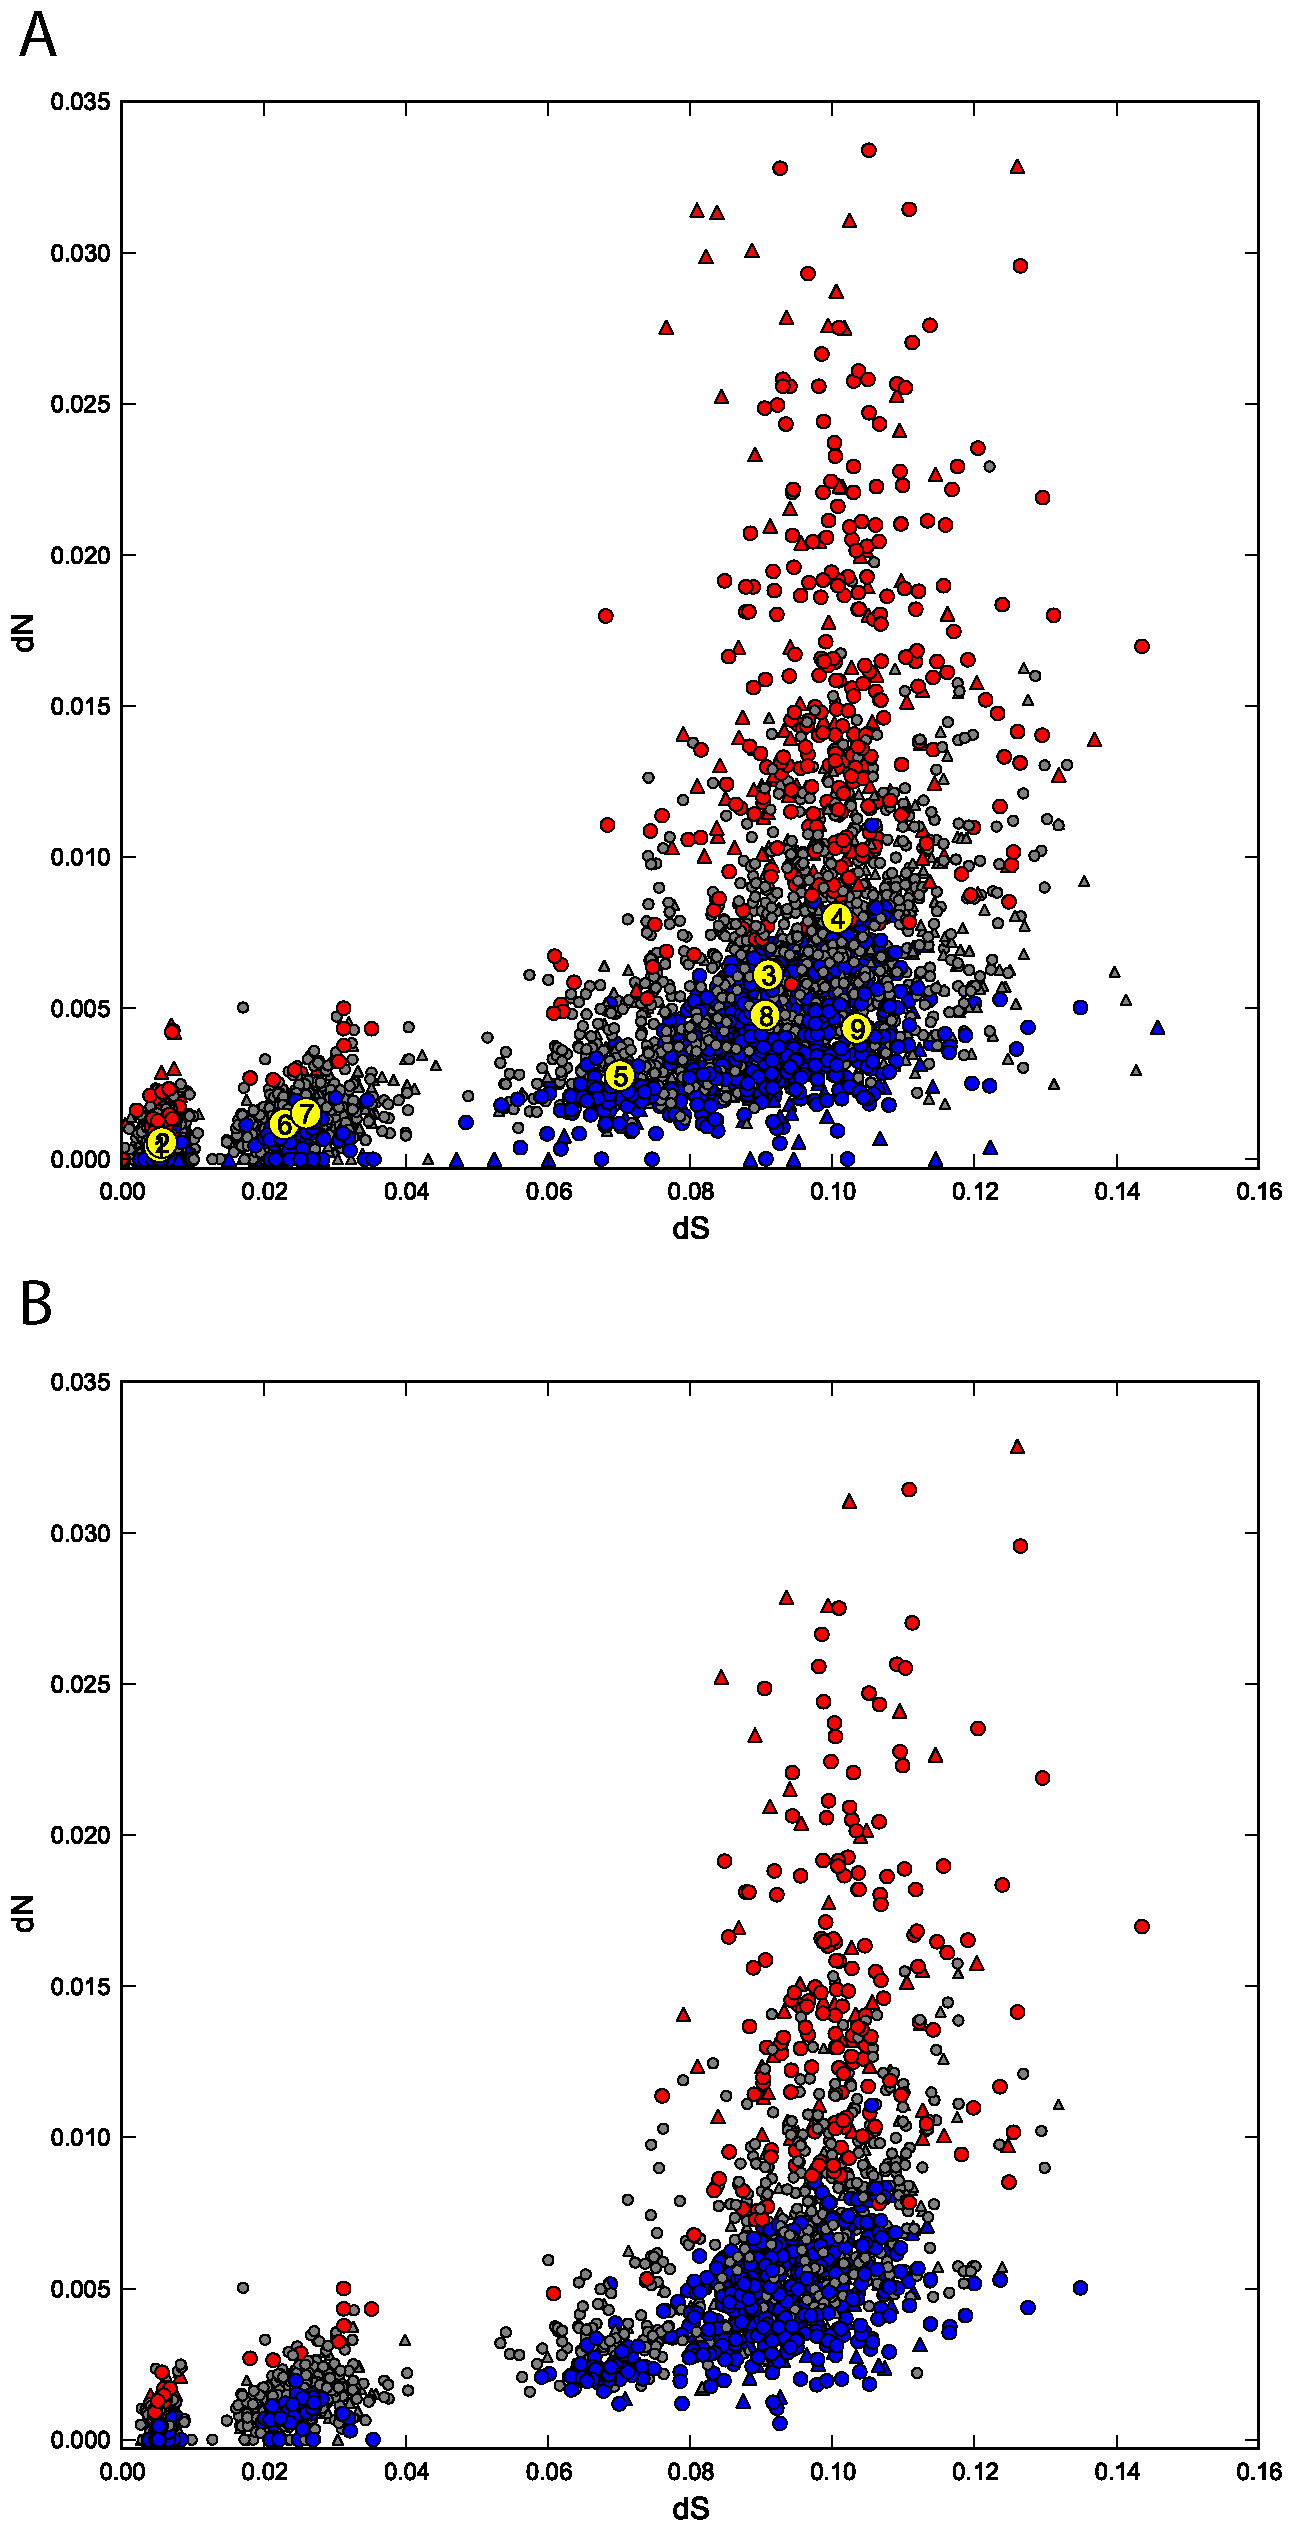
\includegraphics[height=\textheight]{tex_source/figures/gssa/gssa_psgs.png}
\caption[ Positive selection and evolution of functional modules.]{{\bf  Positive selection and evolution of functional modules.} \\Circles and triangles represent the median values of dN and dS for KEGG pathways and GO terms (level 6-7), respectively in mammals, and in the \textit{Drosophila} species. Functional modules with SH$\omega$ and SL$\omega$ results after GSSA are shown in red and blue. Those modules without statistical differences are gray. Yellow dots depict the median dS and dN values for \textit{H. sapiens} (1), \textit{P. troglodytes} (2), \textit{M. musculus} (3), \textit{R. norvegicus} (4), \textit{D. simulans} (5), \textit{D. sechellia} (6), \textit{D. melanogaster} (7), \textit{D. yakuba} (8) and \textit{D. erecta} (9). (B) In this case, circles and triangles represent a subset (of A) with modules containing at least one PSG. Note that they are distributed along a wide range of values of dS and dN and in functional categories with significant (red/blue), and non-significant (gray) results after the GSSA ($\omega$ ratio).} 
\label{fig:gssa_psgs}
\end{FPfigure}

Finally, we ask if PSGs preferentially concentrate in functional modules evolving at faster rates in different genomes. For doing that we computed the mean number of PSGs in functional modules with SH$\omega$ and SL$\omega$ results (red and blue dots in \fref{fig:gssa_psgs}{-B}. As expected, functional modules evolving at high $\omega$ ratio contain higher numbers of PSGs in rodents (p$<$0.001), mammals (p$<$0.001), and \textit{Drosophila} (p$<$0.001) species. For primates however, it was not significant (p = 0.47), indicating that PSGs are distributed almost evenly in functional modules evolving at significantly high and low values of $\omega$ in human and chimpanzee.

To contrast these results, PSGs from previous works in mammal and \textit{Drosophila} species were collected \cite{Clark2007}, \cite{Kosiol2008a}. The pattern of distribution of PSGs in functional modules was in agreement with the mentioned results: significantly skewed (p$<$0.001) towards higher numbers of PSGs in mammals, rodents, and \textit{Drosophila} species, but showing no differences in primates (p = 0.73).

In summary, PSGs are frequently observed in functional modules evolving under a wide range of evolutionary scenarios; however, they concentrate more frequently in functional groups of genes changing at elevated rates in rodents and \textit{Drosophila} species. Alternatively, PSGs were evenly distributed in functional modules changing at the extreme rates of evolution in primates. This observation suggests that a more complex scheme than the cumulative differences of PSGs must rely on the observed adaptive differences in human and chimpanzee genomes. The search for integrative factors taking into account the action of multiple genes other than only those which have been targeted by positive selection \cite{He2010}, could provide a more accurate view for the analysis of the integrated framework underlying adaptation in complete genomes.

\section{Material and Methods}
\label{sec:gssa_mat-met}
\subsection{Orthology prediction}

Complete genomes of 5 mammals species (\textit{Homo sapiens}, \textit{Pan troglodytes}, \textit{Mus musculus}, \textit{Rattus norvegicus} and \textit{Canis familiaris}) where retrieved from \textit{Ensembl} \cite{Flicek2011}. Also orthology prediction between each pair of species possibly done between human and the others was retrieved from \textit{Ensembl Compara} \cite{Vilella2009} using biomart \cite{Kinsella2011} and taking human as \gls{seed} species. Only groups of orthologs \textit{one-to-one} with one representative of each species where kept in the final dataset \fref{fig:phylogeny}{-A}.

\begin{figure}[htpb] 
\centering 
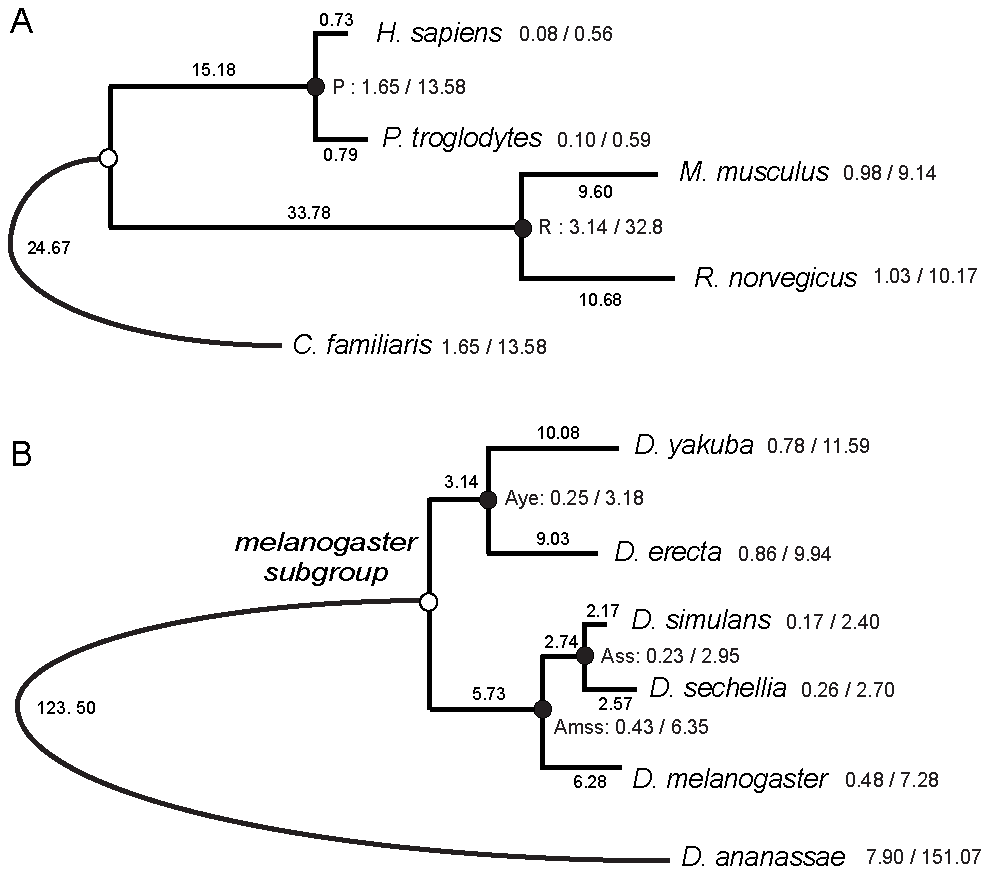
\includegraphics[width=\textwidth]{tex_source/figures/gssa/phylogenies.png}
\caption[Mammals and \textit{Drosophila} phylogeny]{{\bf Mammals and
 \textit{melanogaster} group phylogeny.} \\Numbers on internal and external nodes represent the median number of nonsynonymous and synonymous substitutions per codon (dN/dS) estimated from all the coding sequences compared in mammal (A) and Drosophila (B) genomes. Branch lengths and rates were multiplied by 100. Ancestral estimation of parameters was done in primates (P), rodents (R), D. yakuba and D. erecta (Aye), D. simulans and D. sechellia (Ass), and D. melanogaster, D. simulans and D. sechellia (Amss). C. familiaris and D. ananassae were chosen as outgroup species in the corresponding tree.} 
\label{fig:phylogeny}
\end{figure}


The same procedure was applied for \textit{melanogaster} group, including 6 species namely, \textit{Drosophila melanogaster} (as \gls{seed}-species), \textit{Drosophila sechelia}, \textit{Drosophila simulans}, \textit{Drosophila yakuba}, \textit{Drosophila erecta} and, as outgroup, \textit{Drosophila ananassae} (see \fref{fig:phylogeny}{-B}).

\subsection{Alignments refinement and filters}
DNA coding sequences (CDS) were aligned according to protein translation pattern using \textit{Muscle} version 3.7 \cite{Edgar2004} embedded into the \textit{CDS-Protal} utility in \textit{Phylemon 2.0} \cite{Sanchez2011}, and to avoid the presence of badly aligned regions alignments were cleaned using \textit{TrimAl} \cite{Capella-Gutierrez2009} keeping all sequences but trimming alignment columns with the heuristic method \textit{automated-1}. Additionally, alignments smaller than 100 bp were excluded from the analysis. 

In mammals, the upper limit for dN and dS considered was those of the human interferon $\gamma$ (dN = 3.06) and the relaxin protein \cite{Graur2000} (dS = 6.39 substitutions per site per 1e9 years). Assuming the human-mouse, mouse-rat and human-chimp differentiation times to be about 80, 70 and 5 million years \cite{BlairHedges2003}, respectively, ortholog comparisons between primates and rodents with dS$\ge$1 and dN$\ge$0.5, rodents with dS$\ge$0.256, dN$\ge$0.122, and primates with dS$\ge$0.064 and dN$\ge$0.030 substitutions/site were excluded.

The number of orthologs kept for analysis after filtering steps, is 12,453 for mammals, and 9,240 for flies.

\subsection{Evolutionary analysis}

Maximum likelihood estimation of dN, dS, and $\omega$ was computed using CodeML program from PAML \cite{Yang2007}. Evolutionary rates were computed in orthologous sequences according to the free-ratio branch model assuming independent $\omega$ ratio for each branch of the tree of mammals and Drosophila species (see raw values of rates in Table S1 and S2). Evolutionary rates (dN, dS), its ratio ($\omega$), and its difference between ancestral and descendant species ($\Delta\omega$) were ranked along all genes of genomes and further analyzed by GSSA.

External branches of Figure 1 were labeled as foreground to test for positive selection using branch-site models in Test I and Test II \cite{Zhang2005}. Positive results of relaxation of selective constraints (or weak signals of positive selection) were discarded \cite{Arbiza2006}. To quantify the relative contribution of PSGs in functional modules showing SH$\omega$ and SL$\omega$ results in GSSA, a t-test (from R package \cite{Ihaka1996}) with the mean number of PSGs per functional modules was computed in primates, rodents, mammals and Drosophila species. An independent set of PSGs was collected to test the robustness of our results in mammals \cite{Kosiol2008a}, and Drosophila species \cite{Clark2007}.

\subsection{GSSA, evolutionary and statistical simulations}

Gene-set selection analysis across lists of genes ranked by different evolutionary rate parameters (dS, dN, $\omega$ and $\Delta\omega$) was computed using the program Babelomics \cite{Al-Shahrour2008}. This program implements a version of GSA \cite{Al-Shahrour2005a} which can be applied to any list of ranked genes regardless of the initial experimental design \cite{Dopazo,Huang2009}. The aim of the test is to find functional classes, namely blocks of genes that share some functional property, showing a significant asymmetric distribution towards the extremes of a list of ranked genes. This is achieved by means of a segmentation test, which consists on the sequential application of a Fisher's exact test over the contingency tables formed with the two sides of different partitions (A and B in \fref{fig:gssa_met}) made on an ordered list of genes. The two-tailed Fisher's exact test finds significantly over or under represented functional classes when comparing the upper side to the lower side of the list, as defined by any partition (in \fref{fig:gssa_met}, four of the five partitions show significant differences). Similarly to other equivalent gene-set analyses, the outcomes are those modules (GO and KEGG) significantly associated to high or low values of the evolutionary parameter used to rank the genes. Previous results showed that a number between 20 and 50 partitions often gives optimal results in terms of sensitivity and results recovered \cite{Al-Shahrour2005a}. Here we applied 30 partitions along all the GSSA performed. Given that multiple functional classes (C) are tested in multiple partitions (P), the unadjusted p-values for a total of C $\cdot$ P tests were corrected by the widely accepted FDR method \cite{Benjamini2001}.

\begin{FPfigure}
\centering 
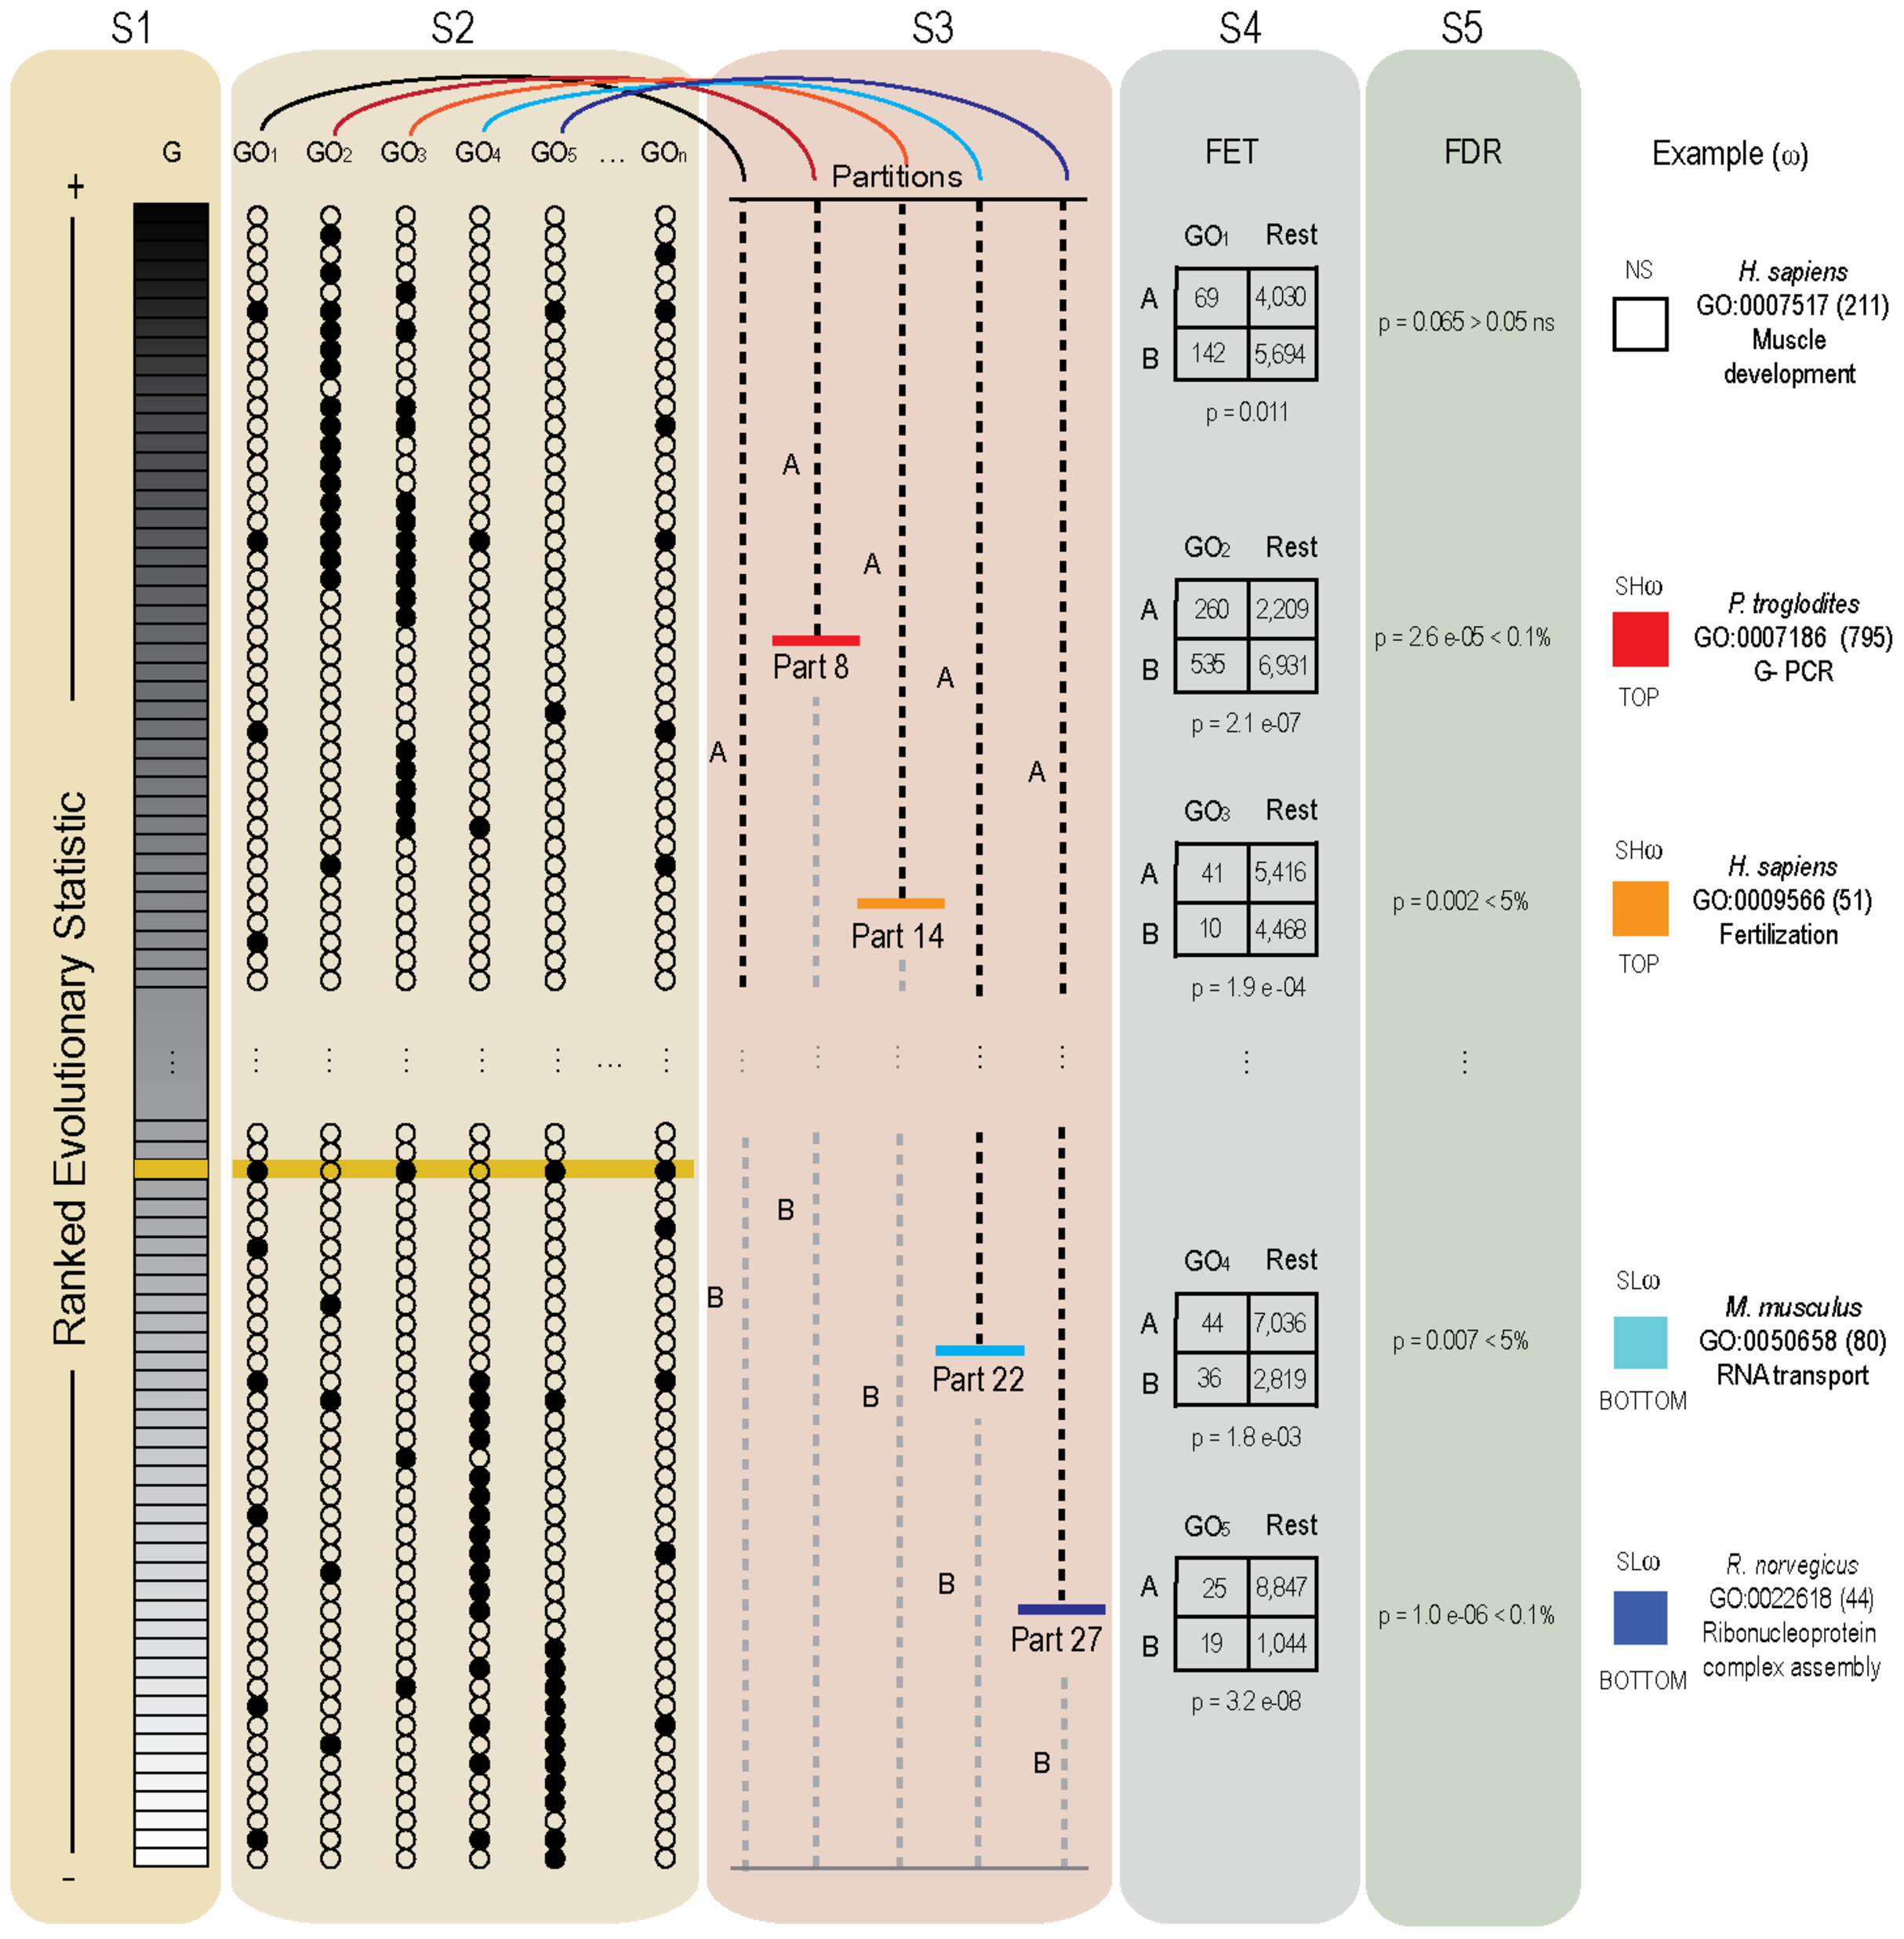
\includegraphics[width=\textwidth]{tex_source/figures/gssa/gssa_met.pdf}
\caption[Summary of the steps developed by the GSSA.]{{\bf Summary of the steps developed by the GSSA.} \\GSSA can be roughly described in a series of five steps (S1 to S5). S1: rank genes of a genome according to an evolutionary variable, S2: assign functional classes to all the listed genes, S3: apply a fixed number of partitions on the ranked list, S4: proceeds with a Fisher exact test (FET) for each partition, S5: adjust p-values by FDR. See text for a full description. Colored boxes (red, orange, cyan and blue) represent functional modules with genes significantly accumulated (0.1\% FDR and 5\% FDR) at the corresponding extremes of a list (top and bottom), and therefore with significantly high (SH) and low (SL) values of the evolutionary variable ($\omega$) respectively. White represents a non-significant association (NS). Examples show five alternative GO categories with significant and non-significant distributions of the $\omega$ statistic. In parenthesis, the total number of genes corresponding to the GO term is shown. For GO1, the function seems to be uncorrelated with the arrangements of the genes. In the example (GO:0007517) partition 16 in human (not shown in the picture) reported the lowest p-value (p = 0.011) although it was not significant after FDR correction (FDR = 0.065). Upper (A) and lower (B) sides of the ranked list (S3) represent both sides of the specified partition number. Remainder GO categories (GO2 to GO5) show the association of dark dots with values located at the top (significant high $\omega$ values -SH$\omega$), and at the bottom (significant low $\omega$ values -SL$\omega$) of the list (for GO2-GO3 and GO4-GO5, respectively). In examples, FETs found the most significant p-value for partitions 8, 14, 22 and 27 for GO:0007517, GO:0007186, GO:0009566, GO:0050658 and GO:0022618 in chimpanzee, human, mouse and rat genome, respectively.}
\label{fig:gssa_met}
\end{FPfigure}

Originally, 1,394/1,331 GO terms, and 199/116 KEGG pathways were analyzed in mammals and Drosophila species respectively. The global GO directed acyclic graph was processed with Blast2GO \cite{Conesa2005} to extend the annotation at missing parental nodes, discarding GO levels out of 2 to 8 for mammals, and 2 to 12 for Drosophilas. The final set of GO and KEGG terms used in the GSSA corresponds to those containing a minimum number of 15 genes. To test possible biases attributed to the size of the functional category, the magnitude of change in evolutionary rate or the proportion of genes experiencing a rate change we randomized the original assignation of ENSG's to the list of ranked values and functional annotation (see \fref{fig:gssa_simul}{-A}). For each evolutionary variable and species 10.000 randomizations and the corresponding GSSA were performed. The proportion of false positives (significant results after GSSA) was computed for each evolutionary variable and plotted along the size of functional categories (from 20 to 1,400 with intervals of 20). Because this proportion never reached values higher than 0.5\% (FDR) we rejected the possibility that either group size or rate distribution biased GSSA results in our data set (see \fref{fig:gssa_simul}{-B} and \fref{fig:gssa_simul}{-C}).

\begin{FPfigure}
\centering 
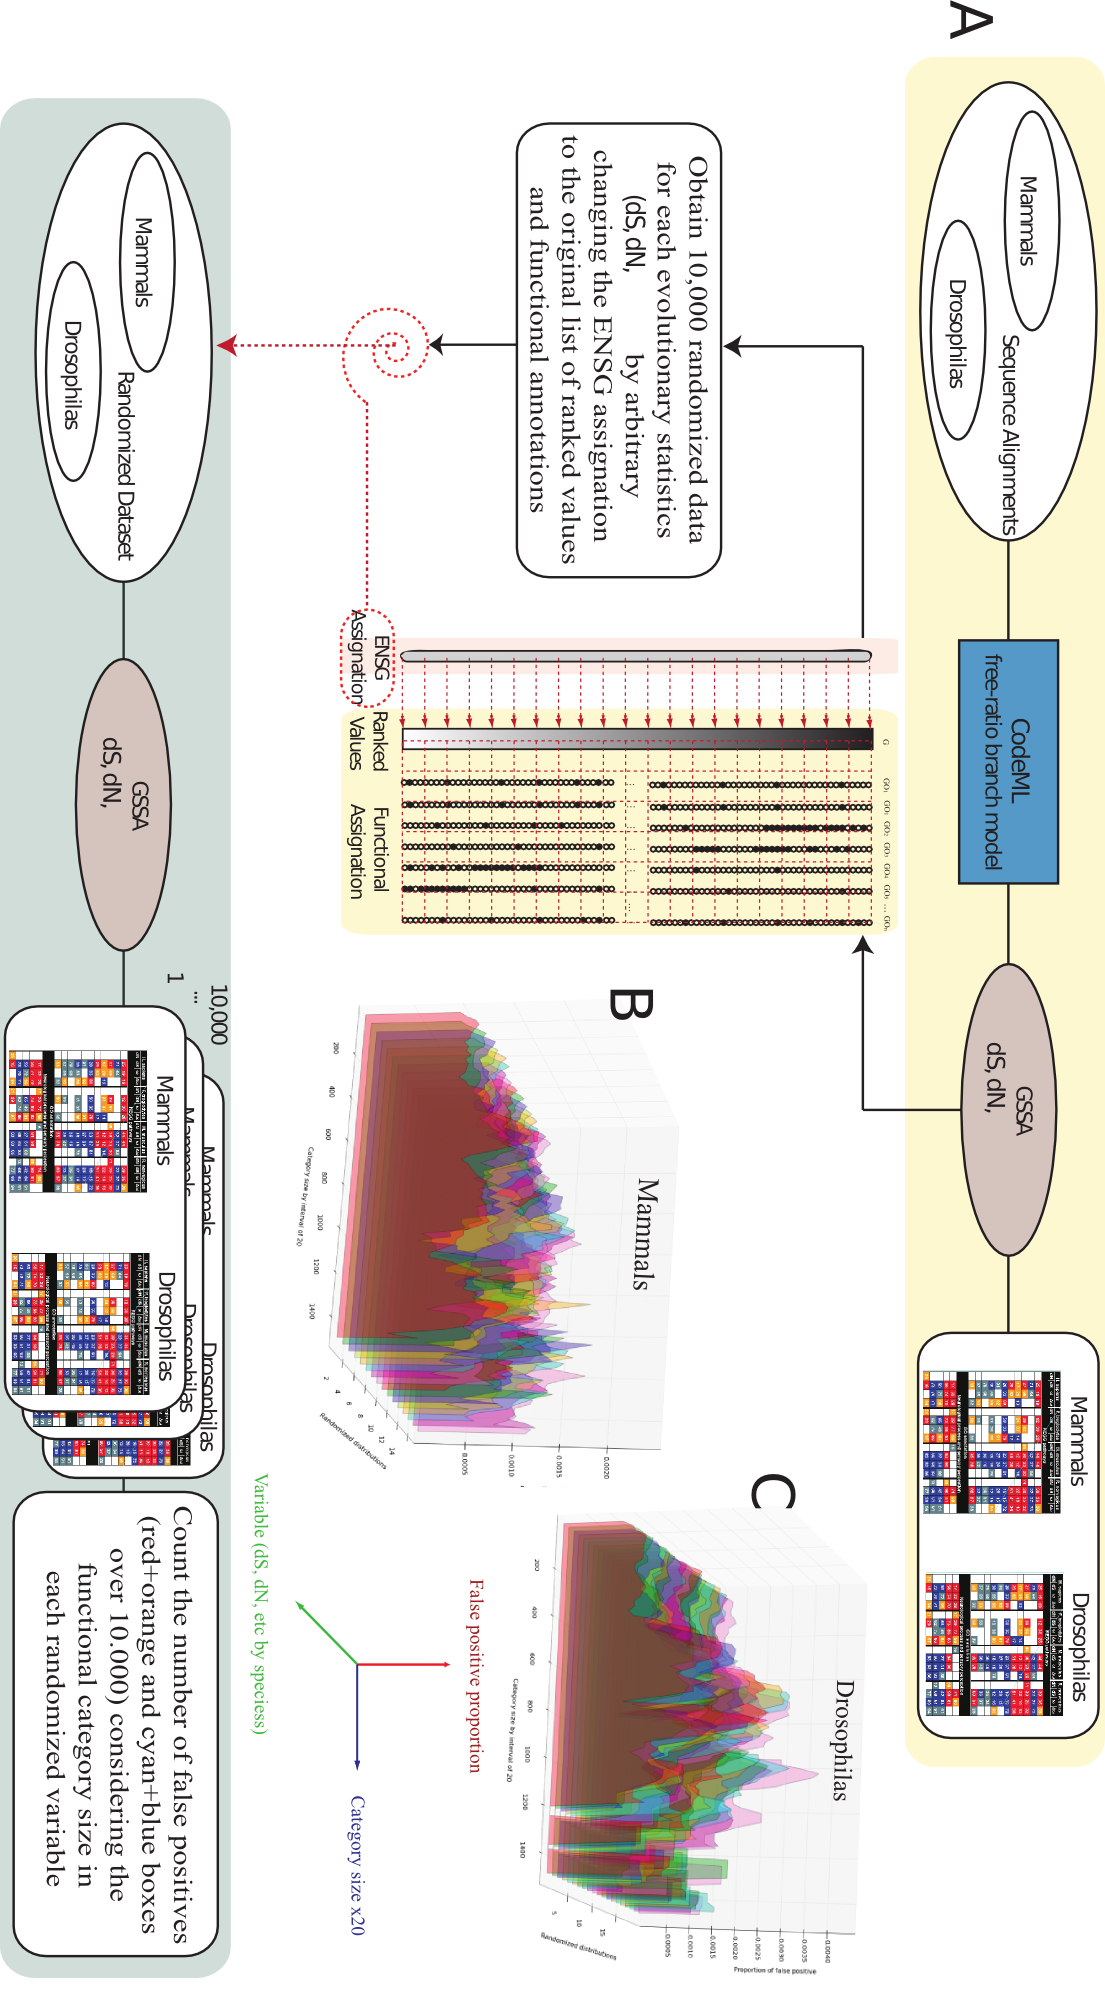
\includegraphics[height=\textheight]{tex_source/figures/gssa/gssa_simulations.png}
\caption[Randomisation experiment.]{{\bf Randomisation experiment.} \\(A) The pipeline shows the steps followed to tests possible biases attributed to the size of the functional category, the magnitude of change in evolutionary rate and the proportion of genes experiencing a rate change in the GSSA. The proportion of false positive results never reached 5\% (FDR) in mammals (B) and Drosophila (C).}
\label{fig:gssa_simul}
\end{FPfigure}

Finally, in order to validate the independence of the GSSA from the effects of alternative evolutionary constraints we simulated selective regimes (purifying selection, positive selection and relaxation of selective constraints) using branch-site models. Here we addressed the possibility of a variation in the representation of significant results after GSSA (see \fref{fig:gssa_simul_pipe}{}). The pipeline described here, shows three different areas: 
\begin{itemize}
\item \textbf{Real Data}: the dark yellow area describes the steps used to reach to results described in the manuscript. The light yellow area describes the use of the CodeML program from PAML package (reference 15 in the ms) to extract -from the original set of sequences -the evolutionary parameters to simulate new sequences under purifying selection (PF), positive selection (PS) and relaxation of the selective constraints (RX) using branch-site models (see model description below). Human, mouse, \textit{D. erecta} and \textit{D. melanogaster} were used as foreground species in the corresponding models.
\item \textbf{Simulated Data}: Evolver (PAML program) simulates sequences using parameters (codon frequencies and branch lengths) from the empirical data. We checked the desired characteristics of positive selection (PS) and relaxation of selective constraints (RX) on the set of the simulated sequences \tref{tab:psg_simul}. Evolutionary variables (dS, dN, $\omega$ and $\Delta\omega$) were estimated from simulated sequences by means of a free-ratio branch model (CodeML). The complete pipeline of the GSSA was applied in the simulated data.
\item \textbf{Testing simulation}: The odd-ratio of the values observed on the contingency table of each significant functional term after GSSA was computed. Values higher and lower than one contribute to the total number of functional modules with significant high and low $\omega$ values. To test the statistical contribution of these functional modules to these extremes on the simulated regimes (PS, RX and PF) the log odd-ratios were compared using t-test.
\end{itemize}

\begin{figure}
\centering 
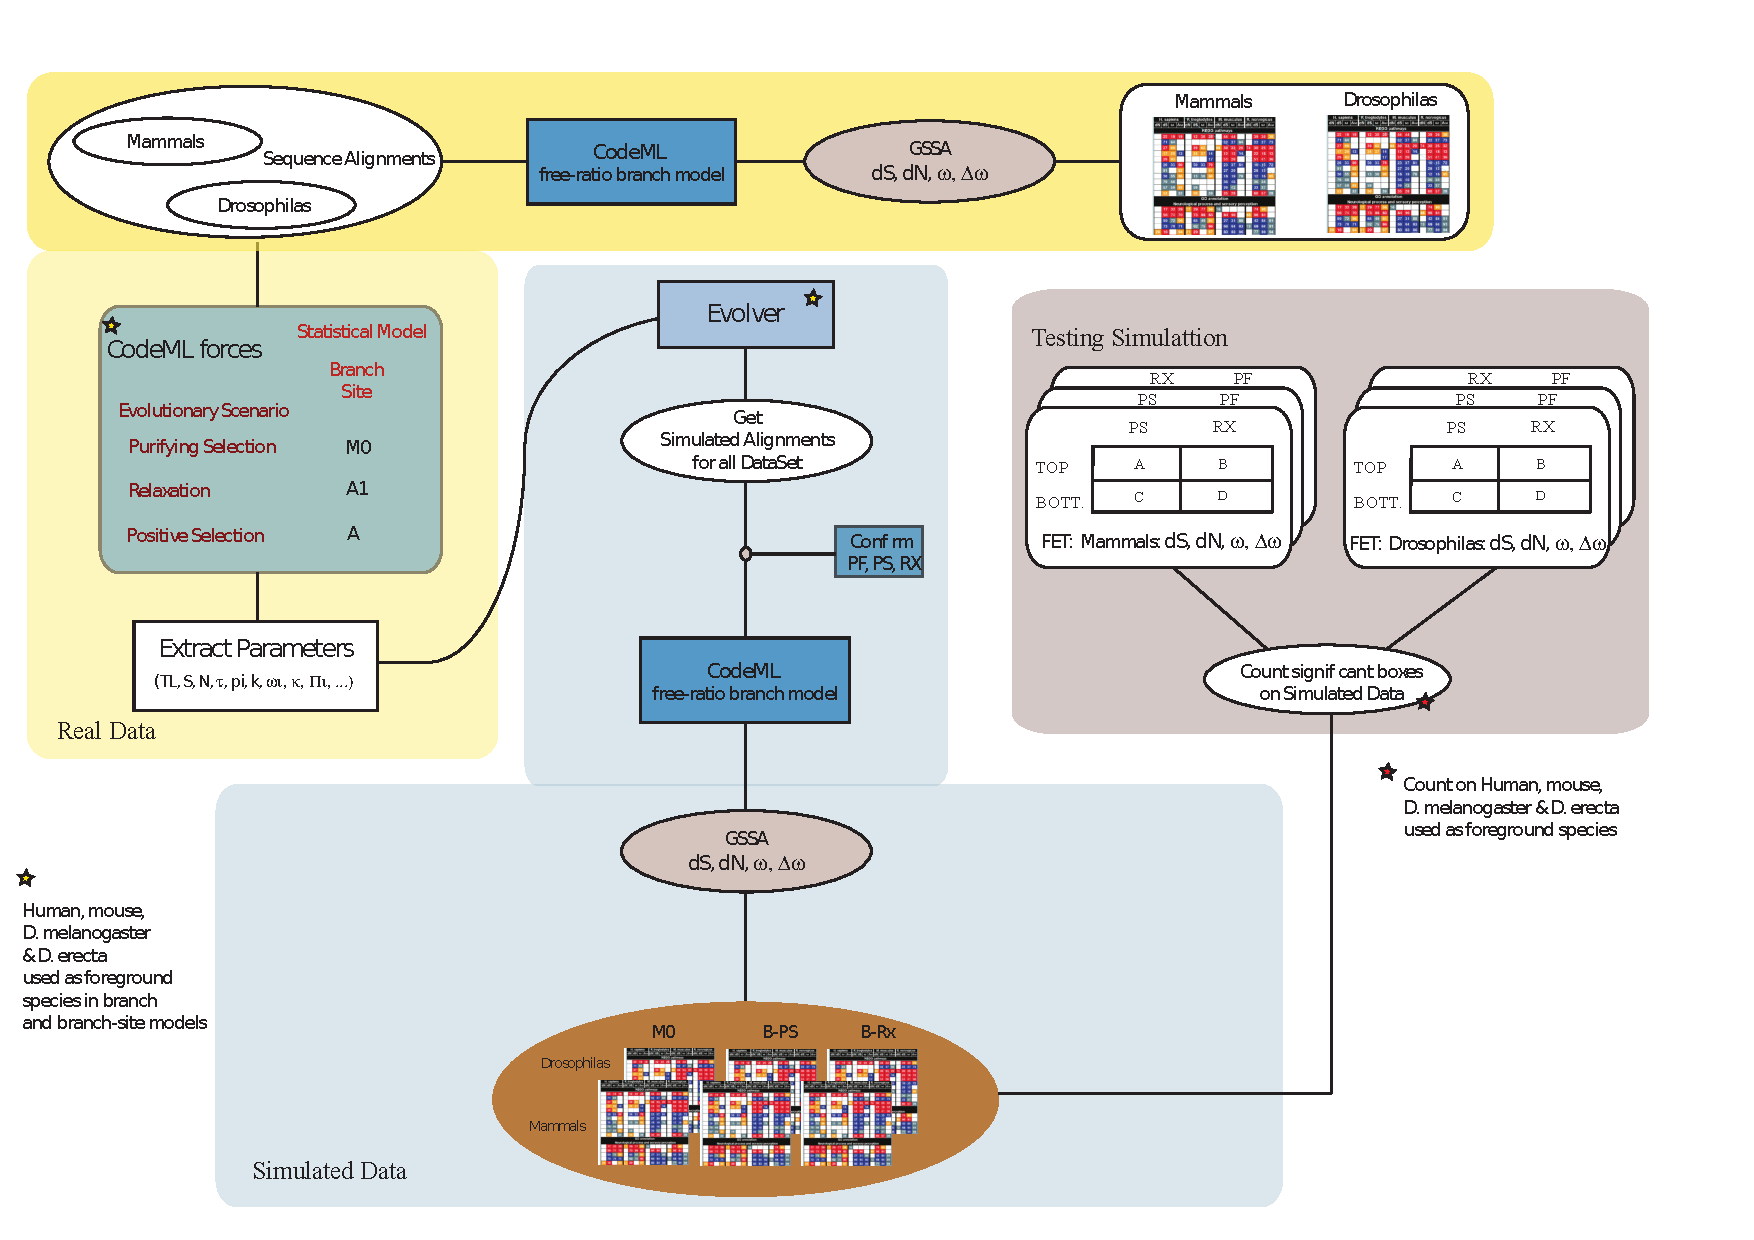
\includegraphics[width=\textwidth]{tex_source/figures/gssa/gssa_simulations_pipeline.pdf}
\caption[Evolutionary and statistical simulation of GSSA.]{{\bf Evolutionary and statistical simulation of GSSA.} \\ The pipeline shows the steps taken along three different spaces of analysis, the real data, the simulated data and the testing block. See Supplementary Results for a complete explanation of methods and results.}
\label{fig:gssa_simul_pipe}
\end{figure}

\rowcolors{1}{white}{white}
\begin{table}[htbp]
\begin{tabular}{l r r r r r r}
\multicolumn{1}{l}{} & \multicolumn{ 2}{c}{PS} & \multicolumn{ 2}{c}{RX} & \multicolumn{ 2}{c}{PF} \\ \hline
\multicolumn{1}{l}{} & \multicolumn{1}{c}{\# PSG} & \multicolumn{1}{c}{\# RXG} & \multicolumn{1}{c}{\# PSG} & \multicolumn{1}{c}{\# RXG} & \multicolumn{1}{c}{\# PSG} & \multicolumn{1}{c}{\# RXG} \\ \hline
Homo sapiens & 658 & 1640 & 11 & 1939 & 0 & 1 \\
Mus musculus & 1500 & 954 & 14 & 1565 & 1 & 0 \\
D. melanogaster & 736 & 630 & 25 & 1104 & 0 & 0 \\
D. erecta & 778 & 1292 & 26 & 1713 & 2 & 1 \\ \hline
\end{tabular}
\caption[Number of PSG and relaxed genes (RXG) in each of the simulated evolutionary scenarios]{Number of PSG and relaxed genes (RXG) in each of the simulated evolutionary scenarios.}
\label{tab:psg_simul}
\end{table}

Our results showed that in spite of the alternative evolutionary scenarios no significant differences were observed between log odd-ratios distribution (p<0.05). This result is exactly what we expected. The average effect of PF, and RX-PS is the proportional decrease and increase of the mean value of $\omega$ on sequences, respectively. This change has minor effects (if any) in the relative position of genes in the ranked list of genes of a genome. Accordingly, since no net differences were produced after ranking genes, no significant differences are expected after the t-test (PS-RX: p= 0.99, PS-PF: p= 0.45, and RX-PF: p= 0.46). The fact that basically the same number of significant results was observed in each evolutionary scenario confirmed this prediction \tref{tab:prop_signif}. We conclude that neither of the selective regimes simulated produce significant differences or biases in the GSSA of $\omega$ values.


\begin{table}[htbp]
\begin{center}
\begin{tabular}{l c c c}
\hline
 & PS & RX & PF \\ \hline
PS & --- & 92.50\% & 98.50\% \\
RX & 91.10\% & --- & 99.00\% \\
PF & 88.90\% & 90.60\% & --- \\ \hline
\end{tabular}
\end{center}
\caption[Proportion of significant functional categories that are still significant.]{Proportion of significant functional categories that are still significant (identical signs of odd-ratios) under a different evolutionary scenario.}
\label{tab:prop_signif}
\end{table}

\section{open on colocalization to not random}

%%% Local Variables: 
%%% mode: latex
%%% TeX-master: "../../master"
%%% End: 
